\documentclass[10.5pt,a4paper]{article}
\usepackage[utf8]{inputenc}
\usepackage[T1]{fontenc}
\usepackage{lmodern}
\usepackage{microtype}
\usepackage[a4paper,margin=18mm,headheight=15pt]{geometry}
\usepackage{amsmath,amssymb,mathtools}
\usepackage{graphicx}
\usepackage{xcolor}
\usepackage{tikz}
\usetikzlibrary{arrows.meta,positioning,calc,shapes.geometric,backgrounds,fit}
\usepackage{booktabs,tabularx,array,multirow}
\usepackage{enumitem}
\usepackage{multicol}
\usepackage{fancyhdr}
\usepackage{titlesec}
\usepackage{caption}
\usepackage{float}
\usepackage{hyperref}
\usepackage{lastpage}

\definecolor{Ink}{HTML}{172033}
\definecolor{Muted}{HTML}{667085}
\definecolor{Panel}{HTML}{F3F5F9}
\definecolor{Rule}{HTML}{D9DEE8}
\definecolor{PR}{HTML}{E53E4D}
\definecolor{PG}{HTML}{16A66A}
\definecolor{PB}{HTML}{2F6FED}
\definecolor{PC}{HTML}{00A7B5}
\definecolor{PM}{HTML}{C13DBA}
\definecolor{PY}{HTML}{D9A400}
\definecolor{Deep}{HTML}{111827}

\hypersetup{colorlinks=true,linkcolor=PB,urlcolor=PB,citecolor=PB,pdftitle={Percepta Technical Manual},pdfauthor={Virgile Adam}}
\setlength{\parindent}{0pt}
\setlength{\parskip}{5pt}
\setlist[itemize]{leftmargin=5mm,itemsep=2pt,topsep=3pt}
\setlist[enumerate]{leftmargin=6mm,itemsep=2pt,topsep=3pt}
\renewcommand{\arraystretch}{1.18}
\captionsetup{font=small,labelfont=bf,textfont={color=Muted}}
\pagestyle{fancy}
\fancyhf{}
\fancyhead[L]{\small\color{Muted}PERCEPTA / TECHNICAL MANUAL}
\fancyhead[R]{\small\color{Muted}v0.31.0}
\fancyfoot[L]{\small\color{Muted}\copyright\ 2026 Virgile Adam}
\fancyfoot[R]{\small\color{Muted}\thepage\ / \pageref{LastPage}}
\renewcommand{\headrulewidth}{0.4pt}
\renewcommand{\headrule}{\hbox to\headwidth{\color{Rule}\leaders\hrule height \headrulewidth\hfill}}
\titleformat{\section}{\Large\bfseries\color{Ink}}{\thesection}{0.65em}{}
\titleformat{\subsection}{\large\bfseries\color{Ink}}{\thesubsection}{0.6em}{}
\titleformat{\subsubsection}{\normalsize\bfseries\color{Ink}}{\thesubsubsection}{0.55em}{}
\titlespacing*{\section}{0pt}{12pt}{5pt}
\titlespacing*{\subsection}{0pt}{9pt}{3pt}

\newcommand{\RGBbar}{\textcolor{PR}{\rule{0.32\linewidth}{2.3pt}}\hspace{-1pt}\textcolor{PG}{\rule{0.32\linewidth}{2.3pt}}\hspace{-1pt}\textcolor{PB}{\rule{0.32\linewidth}{2.3pt}}}
\newcommand{\note}[1]{\vspace{3pt}\noindent\colorbox{Panel}{\parbox{0.965\linewidth}{\small\textbf{Note.} #1}}\vspace{3pt}}
\newcommand{\tip}[1]{\vspace{3pt}\noindent\fcolorbox{PB}{white}{\parbox{0.95\linewidth}{\small\textbf{Practical tip.} #1}}\vspace{3pt}}
\newcommand{\code}[1]{\texttt{#1}}
\newcommand{\clip}{\operatorname{clip}}
\newcommand{\mean}{\operatorname{mean}}

\begin{document}

% COVER
\thispagestyle{empty}

\begin{tikzpicture}[remember picture,overlay]
  \fill[Deep] (current page.south west) rectangle (current page.north east);
  \fill[PR] ([xshift=0mm,yshift=-20mm]current page.north west) rectangle ([xshift=70mm,yshift=-23mm]current page.north west);
  \fill[PG] ([xshift=70mm,yshift=-20mm]current page.north west) rectangle ([xshift=140mm,yshift=-23mm]current page.north west);
  \fill[PB] ([xshift=140mm,yshift=-20mm]current page.north west) rectangle ([xshift=210mm,yshift=-23mm]current page.north west);
  \begin{scope}[shift={([xshift=105mm,yshift=-112mm]current page.north west)}]
    \foreach \x in {-58,-48,...,58}{
      \draw[PR,line width=2.0pt,opacity=.78] (\x,-34) -- (\x,34);
      \draw[PG,line width=2.0pt,opacity=.78] (\x+2.2,-34) -- (\x+2.2,34);
      \draw[PB,line width=2.0pt,opacity=.78] (\x+4.4,-34) -- (\x+4.4,34);
    }
    \foreach \r in {4,8,...,34}{
      \draw[white,opacity=.13,line width=.4pt] (0,0) circle (\r);
    }
    \draw[white,line width=.8pt,opacity=.5] plot[smooth,domain=0:21,samples=500] ({.56*\x*cos(\x r)},{.56*\x*sin(\x r)});
  \end{scope}
\end{tikzpicture}
\vspace*{40mm}
{\color{white}\fontsize{34}{38}\selectfont\bfseries PERCEPTA\par}
\vspace{3mm}
{\color{white}\Large Technical Manual\par}
\vspace{2mm}
{\color{white!68}\large Perceptual pattern image generator\par}
\vfill
\begin{minipage}{0.78\linewidth}
{\color{white!82}\large Algorithms, visual perception model, parameter semantics, animation and export}\par
\vspace{8mm}
{\color{white!58}Version 0.31.0 \quad | \quad July 2026}\par
\vspace{3mm}
{\color{white!58}Virgile Adam --- IBS, CNRS, Universit\'e Grenoble Alpes}\par
\end{minipage}
\vspace*{20mm}
\clearpage

\section*{About this manual}
\addcontentsline{toc}{section}{About this manual}
Percepta converts a conventional RGB image into a geometric pattern made of coloured stripes, dots or a continuous spiral. Close to the image, the geometry is explicit. At a greater viewing distance, spatial averaging by the display, the optics and the visual system reveals the source image.

This manual describes the user-facing workflow and the mathematical model implemented by the current Percepta renderers. It is deliberately compact: it explains every control that materially changes the result, gives the equations behind each pattern family, and provides practical guidance for screen display, animation and print.

\note{The perceptual model used here is an engineering approximation, not a clinical model of human vision. The effective fusion distance depends on the observer, output size, display or print process, ambient light and contrast.}

\begin{center}\RGBbar\end{center}
\tableofcontents
\vfill
\begin{tabularx}{\linewidth}{@{}lX@{}}
\toprule
Document & Percepta Technical Manual \\
Software & Percepta 0.31.0 \\
Author & Virgile Adam \\
Contact & \href{mailto:virgile.adam@ibs.fr}{virgile.adam@ibs.fr} \\
Web & \href{https://www.virgile-adam.com}{www.virgile-adam.com} \\
Project & \href{https://github.com/VirgileAdam/Percepta}{github.com/VirgileAdam/Percepta} \\
Copyright & \copyright\ 2026 Virgile Adam \\
\bottomrule
\end{tabularx}
\clearpage

\section{Purpose and workflow}
\subsection{What Percepta produces}
Percepta does not reproduce the source image as a conventional grid of coloured pixels. Instead, each colour channel controls the local geometry of a red, green or blue structure. The average colour of a neighbourhood is preserved while its spatial distribution is reorganised into a visible pattern.

The six renderers are:
\begin{multicols}{2}
\begin{itemize}
\item Vertical stripes
\item Horizontal stripes
\item Diagonal stripes
\item Halftone
\item Hexagonal halftone
\item Spiral stripes
\end{itemize}
\end{multicols}

\subsection{End-to-end pipeline}
\begin{figure}[H]
\centering
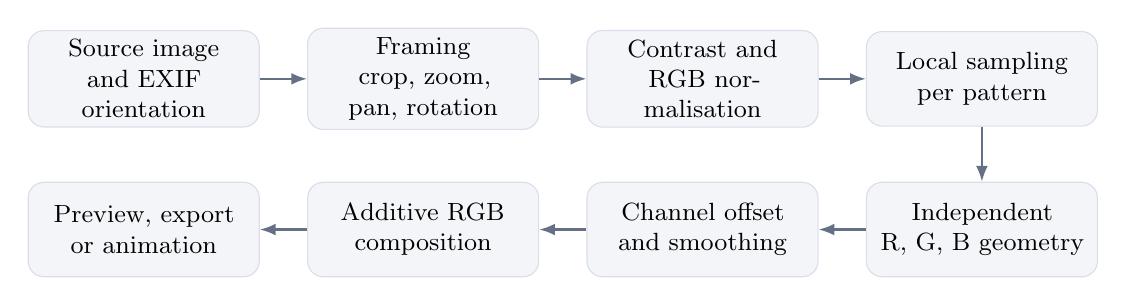
\begin{tikzpicture}[node distance=7mm and 6mm, every node/.style={font=\small}, box/.style={draw=Rule,rounded corners=2mm,fill=Panel,minimum height=12mm,text width=27mm,align=center}, arr/.style={-{Latex[length=2mm]},thick,draw=Muted}]
\node[box] (a) {Source image\\and EXIF orientation};
\node[box,right=of a] (b) {Framing\\crop, zoom, pan, rotation};
\node[box,right=of b] (c) {Contrast and\\RGB normalisation};
\node[box,right=of c] (d) {Local sampling\\per pattern};
\node[box,below=of d] (e) {Independent\\R, G, B geometry};
\node[box,left=of e] (f) {Channel offset\\and smoothing};
\node[box,left=of f] (g) {Additive RGB\\composition};
\node[box,left=of g] (h) {Preview, export\\or animation};
\draw[arr] (a)--(b); \draw[arr] (b)--(c); \draw[arr] (c)--(d);
\draw[arr] (d)--(e); \draw[arr] (e)--(f); \draw[arr] (f)--(g); \draw[arr] (g)--(h);
\end{tikzpicture}
\caption{Processing pipeline. Each renderer changes the local sampling and geometry stage, while framing, colour processing, composition and export are shared.}
\end{figure}

\subsection{Five-minute workflow}
\begin{enumerate}
\item Select \textbf{Open image} and choose a photograph or illustration.
\item Use \textbf{Framing} to choose the crop ratio, then adjust zoom, pan and rotation.
\item Select a pattern. Start with the adaptive default density.
\item Adjust \textbf{Strength}, \textbf{Colour separation} and \textbf{Source contrast}.
\item Select the output size and press \textbf{Generate}.
\item Inspect the result both close up and reduced on screen. Export the still image or create a density animation.
\end{enumerate}

\tip{Judge recognisability at several zoom levels. A pattern that looks too abstract at 100\% may reconstruct clearly when the preview is reduced to 15--30\%.}

\section{Interface and controls}
\subsection{Workspace anatomy}
The workspace is organised around a compact control panel and two large previews. The source preview shows the framed input. The generated preview shows the encoded result. The status line reports the selected pattern and output dimensions. Animation controls run along the lower edge so density motion can be tested without leaving the main workspace.

\begin{figure}[H]
\centering
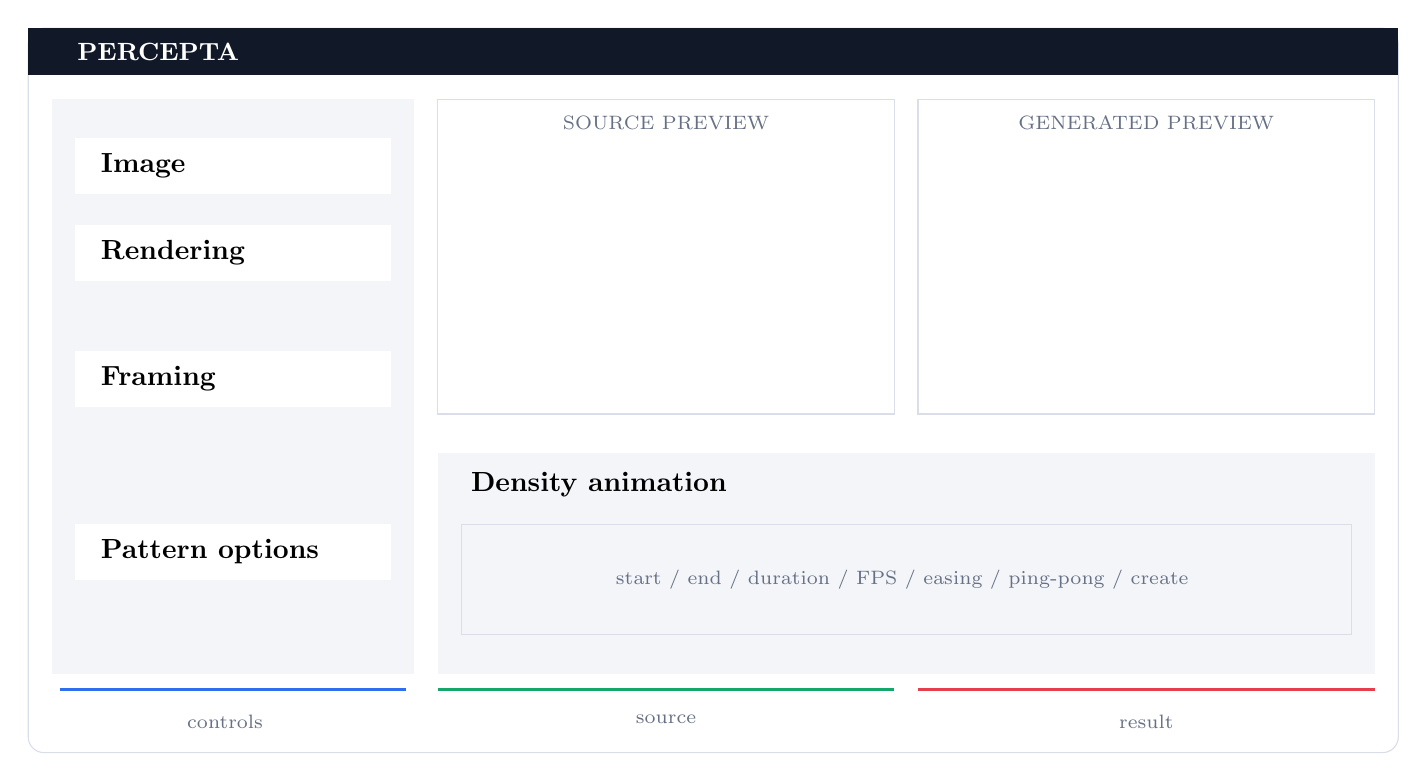
\begin{tikzpicture}[x=1mm,y=1mm,font=\scriptsize]
\draw[rounded corners=2mm,fill=white,draw=Rule] (0,0) rectangle (174,92);
\fill[Deep] (0,86) rectangle (174,92);
\node[anchor=west,text=white,font=\bfseries\small] at (5,89) {PERCEPTA};
\fill[Panel] (3,10) rectangle (49,83);
\draw[Rule] (52,43) rectangle (110,83);
\draw[Rule] (113,43) rectangle (171,83);
\node[Muted] at (81,80) {SOURCE PREVIEW};
\node[Muted] at (142,80) {GENERATED PREVIEW};
\foreach \y/\t in {78/Image,67/Rendering,51/Framing,29/Pattern options}{
  \draw[white,fill=white] (6,\y-7) rectangle (46,\y);
  \node[anchor=west,font=\bfseries] at (8,\y-3.5) {\t};
}
\fill[Panel] (52,10) rectangle (171,38);
\node[anchor=west,font=\bfseries] at (55,34) {Density animation};
\draw[Rule] (55,15) rectangle (168,29);
\node[Muted] at (111,22) {start / end / duration / FPS / easing / ping-pong / create};
\draw[PB,very thick] (4,8)--(48,8);
\draw[PG,very thick] (52,8)--(110,8);
\draw[PR,very thick] (113,8)--(171,8);
\node[anchor=north,Muted] at (25,6) {controls};
\node[anchor=north,Muted] at (81,6) {source};
\node[anchor=north,Muted] at (142,6) {result};
\end{tikzpicture}
\caption{Schematic map of the main window. The distributed documentation package also contains the original screenshots supplied for each renderer.}
\end{figure}

\subsection{Common rendering controls}
\begin{tabularx}{\linewidth}{@{}>{\bfseries}p{31mm}p{29mm}X@{}}
\toprule
Control & Reference default & Effect \\
\midrule
Pattern & Vertical stripes & Selects the renderer and changes the density label and pattern-specific options. \\
Density & Pattern dependent & Controls stripe count, dot spacing or spiral turn spacing. \\
Strength & 0.80 & Scales the conversion from local channel intensity to geometric width or area. \\
Colour separation & 10 px & Offsets the red, green and blue structures, revealing coloured fringes. \\
Source contrast & 1.55 & Applies contrast before local measurement. \\
Output size & 1600 px & Sets the square output resolution and the scale used by adaptive defaults. \\
Generate & --- & Recomputes the current still image. \\
Export & --- & Saves the generated image in a supported still-image format. \\
\bottomrule
\end{tabularx}

\subsection{Framing}
The crop stage is non-destructive. It is recomputed from the original source whenever a framing control changes.

\begin{itemize}
\item \textbf{Crop} selects a target composition such as Square, Portrait 4:5 or Landscape 4:3.
\item \textbf{Zoom} reduces the sampled region around the current centre.
\item \textbf{Pan X / Pan Y} moves that centre within the available source area.
\item \textbf{Rotation} rotates the source before cropping, using high-quality interpolation and an expanded canvas.
\item \textbf{Reset} restores the neutral framing values.
\end{itemize}

After cropping, the result is fitted into the square render canvas without anisotropic distortion. Any necessary padding is black.

\section{Image preparation and common mathematics}
\subsection{Normalised RGB representation}
After framing and contrast adjustment, the image is represented as three normalised fields:
\begin{equation}
\mathbf{I}(x,y)=
\begin{bmatrix}
I_R(x,y)\\[2pt] I_G(x,y)\\[2pt] I_B(x,y)
\end{bmatrix},
\qquad 0\le I_c(x,y)\le 1,
\qquad c\in\{R,G,B\}.
\end{equation}

A useful analytical representation of the contrast operation is
\begin{equation}
I'_c(x,y)=\clip\!\left(\mu_c+C\,[I_c(x,y)-\mu_c],\,0,\,1\right),
\end{equation}
where $C$ is \textbf{Source contrast} and $\mu_c$ is a channel reference level. The application uses the image-library contrast operator; the equation explains its visual effect: values are expanded away from a neutral level when $C>1$ and compressed when $C<1$.

\subsection{Luminance and automatic pattern selection}
For operations requiring a scalar greyscale field, Percepta uses the standard linear combination
\begin{equation}
L(x,y)=0.2126\,I_R(x,y)+0.7152\,I_G(x,y)+0.0722\,I_B(x,y).
\end{equation}

The automatic selector evaluates a downsampled greyscale image $G$ through a simple detail score:
\begin{equation}
D=\mean_{i,j}\left|G_{i+1,j}-G_{i,j}\right|
 +\mean_{i,j}\left|G_{i,j+1}-G_{i,j}\right|.
\end{equation}
A high score favours halftone; a lower score favours vertical stripes. This heuristic is fast and intentionally conservative. Manual selection remains preferable when the artistic character matters more than local detail.

\subsection{Independent colour masks}
Each renderer creates three masks $M_R$, $M_G$ and $M_B$. The digital output is
\begin{equation}
\mathbf{O}(x,y)=
\begin{bmatrix}
M_R(x,y)\\[2pt]M_G(x,y)\\[2pt]M_B(x,y)
\end{bmatrix}.
\end{equation}
Where all masks overlap, the result is white. Pairwise overlap gives additive secondary colours:
\begin{equation}
R+G=Y,\qquad G+B=C,\qquad R+B=M,\qquad R+G+B=W.
\end{equation}

Colour separation assigns signed offsets
\begin{equation}
\delta_R=-d,\qquad \delta_G=0,\qquad \delta_B=+d,
\end{equation}
where $d$ is the user parameter in output pixels. The exact direction of the offset depends on the renderer: perpendicular to lines, along the halftone grid axis, or along the spiral normal.

\subsection{Spatial averaging model}
At a reduced scale, each channel may be modelled as a convolution with an effective point-spread function $h$:
\begin{equation}
P_c(x,y)=\iint_{\mathbb{R}^2} M_c(u,v)\,h(x-u,y-v)\,\mathrm{d}u\,\mathrm{d}v.
\end{equation}
The design goal is local area consistency:
\begin{equation}
\frac{1}{|\Omega|}\iint_{\Omega}M_c(x,y)\,\mathrm{d}x\,\mathrm{d}y
\approx
\frac{1}{|\Omega|}\iint_{\Omega}I_c(x,y)\,\mathrm{d}x\,\mathrm{d}y.
\end{equation}
Thus, geometric occupancy acts as an analogue code for channel intensity.

\clearpage
\section{Stripe renderers}
\subsection{Vertical stripes}
For a square output of width $N$ pixels and $n$ stripes, the nominal period is
\begin{equation}
P=\frac{N}{n}.
\end{equation}
Stripe centres are placed at
\begin{equation}
x_k=\left(k+\frac{1}{2}\right)P,\qquad k=0,1,\ldots,n-1.
\end{equation}
For each centre, the source is locally averaged over a band approximately $0.60P$ wide. After optional one-dimensional smoothing, local channel intensity controls stripe width:
\begin{equation}
\boxed{
 w_c(y)=w_{\min}+\left(w_{\max}-w_{\min}\right)
 \clip\!\left(S\,[\widetilde I_c(y)]^{\gamma},0,1\right)
}
\end{equation}
with
\begin{equation}
\gamma=0.82,\qquad
w_{\max}=0.66P,\qquad
w_{\min}=\max(1,0.018P).
\end{equation}
The exponent below one lifts moderate intensities, preserving facial and tonal information that could otherwise disappear in narrow structures.

\begin{figure}[H]
\centering
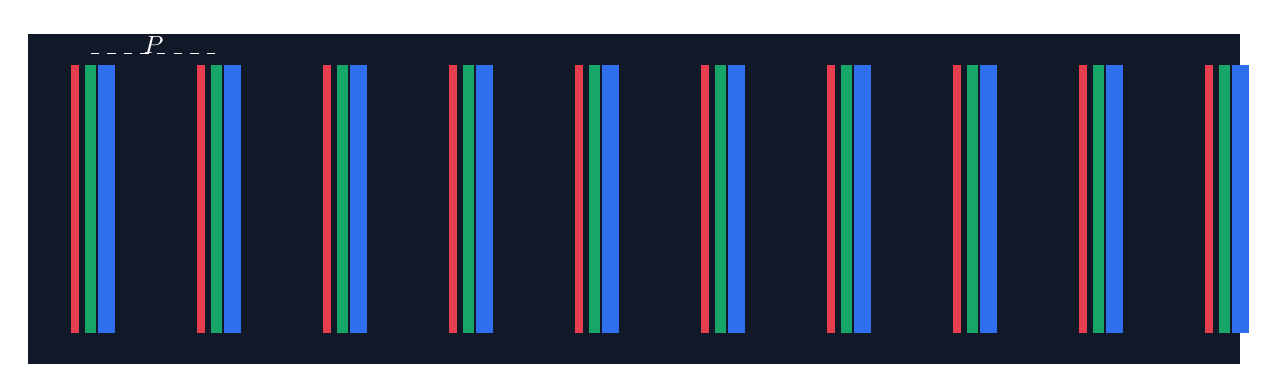
\begin{tikzpicture}[x=1mm,y=1mm]
\fill[Deep] (0,0) rectangle (154,42);
\foreach \x in {8,24,...,152}{
  \draw[PR,line width=2.7pt] (\x-2,4)--(\x-2,38);
  \draw[PG,line width=4.0pt] (\x,4)--(\x,38);
  \draw[PB,line width=6.0pt] (\x+2,4)--(\x+2,38);
}
\draw[white,dashed] (8,39.5)--(24,39.5);
\node[white,font=\small] at (16,40.5) {$P$};
\end{tikzpicture}
\caption{Stripe period is fixed by density; local RGB intensity changes the three channel widths.}
\end{figure}

\subsection{Horizontal stripes}
Horizontal stripes use the same equations after transposition of the source and output axes. This is algorithmically equivalent to applying the vertical renderer to a $90^\circ$-rotated image and rotating the result back.

\subsection{Diagonal stripes}
The source is expanded and rotated by $45^\circ$, encoded with the vertical-stripe engine, then rotated back and centre-cropped. The enlarged intermediate canvas avoids clipping at the corners. A pattern-specific density compensation maintains a useful visual pitch after the diagonal transform.

\subsection{Line smoothing}
The line option applies a moving average along the sampled intensity profile. For integer radius $m$,
\begin{equation}
\widetilde I_c(k)=\frac{1}{2m+1}\sum_{j=-m}^{m}I_c(k+j).
\end{equation}
Higher smoothing suppresses small width fluctuations and produces calmer lines; lower smoothing follows fine texture more closely.

\begin{tabularx}{\linewidth}{@{}lXXX@{}}
\toprule
Pattern & Best suited to & Typical strength & Main risk \\
\midrule
Vertical & Portraits, centred subjects & 0.65--0.95 & Fine horizontal features may weaken. \\
Horizontal & Landscapes, layered scenes & 0.65--0.95 & Thin vertical features may break. \\
Diagonal & Dynamic compositions, architecture & 0.60--0.90 & Rotation can emphasise stair-stepping at low resolution. \\
\bottomrule
\end{tabularx}

\section{Halftone renderers}
\subsection{Square-grid halftone}
The halftone renderer samples the image on a regular grid with spacing $p$. For grid indices $(i,j)$,
\begin{equation}
x_{i,j}=ip,\qquad y_{i,j}=jp.
\end{equation}
The mean channel intensity $\bar I_{c,i,j}$ in the local cell determines the dot radius:
\begin{equation}
\boxed{
r_{c,i,j}=\max\!\left(r_{\min},\,0.47p\sqrt{\clip(S\bar I_{c,i,j},0,1)}\right)
}
\end{equation}
The square root is essential because disk area is proportional to $r^2$:
\begin{equation}
A_{c,i,j}=\pi r_{c,i,j}^{\,2}\propto \bar I_{c,i,j}.
\end{equation}
Thus, once the dots are spatially averaged, area coverage approximately recovers source intensity.

\subsection{Hexagonal halftone}
The hexagonal lattice uses
\begin{equation}
y_j=j\frac{\sqrt{3}}{2}p,
\end{equation}
with alternate rows shifted by half a cell:
\begin{equation}
x_{i,j}=ip+\frac{p}{2}(j\bmod 2).
\end{equation}
This gives six equidistant neighbours and reduces directional bias relative to a square lattice.

\begin{figure}[H]
\centering
\begin{tikzpicture}[x=1mm,y=1mm]
\begin{scope}
\node[font=\bfseries] at (35,38) {Square};
\foreach \x in {8,20,...,62}\foreach \y in {5,17,29}{
 \fill[PR,opacity=.8] (\x-1.6,\y) circle (2.8);
 \fill[PG,opacity=.8] (\x,\y) circle (2.8);
 \fill[PB,opacity=.8] (\x+1.6,\y) circle (2.8);
}
\end{scope}
\begin{scope}[xshift=82mm]
\node[font=\bfseries] at (35,38) {Hexagonal};
\foreach \row/\y in {0/5,1/15.4,2/25.8}{
 \foreach \x in {8,20,...,62}{
  \fill[PR,opacity=.8] (\x+6*mod(\row,2)-1.6,\y) circle (2.8);
  \fill[PG,opacity=.8] (\x+6*mod(\row,2),\y) circle (2.8);
  \fill[PB,opacity=.8] (\x+6*mod(\row,2)+1.6,\y) circle (2.8);
 }
}
\end{scope}
\end{tikzpicture}
\caption{Square and hexagonal sampling. Channel offsets expose RGB fringes while overlap preserves neutral tones.}
\end{figure}

\subsection{Pattern options}
\begin{itemize}
\item \textbf{Dot shape} selects the geometric glyph used by the current build.
\item \textbf{Angle} rotates the sampling field before encoding.
\item \textbf{Minimum size} prevents dark regions from collapsing to invisible points.
\end{itemize}

\tip{If the image becomes too dark, increase minimum size or strength. If neighbouring dots merge into broad solid areas, increase dot spacing or reduce strength.}

\clearpage
\section{Spiral renderer}
\subsection{Archimedean path}
The spiral renderer uses one continuous Archimedean spiral. Let the requested turn spacing be $p$. Then
\begin{equation}
r(\theta)=a+b\theta,
\qquad
b=\frac{p}{2\pi}.
\end{equation}
With centre $(x_0,y_0)$ and direction $q\in\{-1,+1\}$,
\begin{equation}
\begin{aligned}
x(\theta)&=x_0+r(\theta)\cos(q\theta),\\
y(\theta)&=y_0+r(\theta)\sin(q\theta).
\end{aligned}
\end{equation}
The \textbf{Centre X} and \textbf{Centre Y} controls define $(x_0,y_0)$ as percentages of the output dimensions. \textbf{Clockwise} changes the sign of $q$.

\subsection{Normal direction and RGB separation}
Differentiating the path gives a tangent vector
\begin{equation}
\mathbf{t}(\theta)=
\begin{bmatrix}
x'(\theta)\\y'(\theta)
\end{bmatrix}.
\end{equation}
A unit normal is
\begin{equation}
\mathbf{n}(\theta)=
\frac{1}{\sqrt{x'(\theta)^2+y'(\theta)^2}}
\begin{bmatrix}
-y'(\theta)\\x'(\theta)
\end{bmatrix}.
\end{equation}
The channel paths are displaced along this normal:
\begin{equation}
\mathbf{s}_c(\theta)=
\begin{bmatrix}x(\theta)\\y(\theta)\end{bmatrix}
+\delta_c\,\mathbf{n}(\theta),
\qquad c\in\{R,G,B\}.
\end{equation}
Separation is constrained relative to turn spacing so adjacent channel paths do not jump across neighbouring turns.

\subsection{Width modulation}
The source image is sampled along the spiral. After path smoothing, the local width follows the same perceptual response used for stripes:
\begin{equation}
w_c(\theta)=w_{\min}+(w_{\max}-w_{\min})
\clip\!\left(S[\widetilde I_c(\theta)]^{0.82},0,1\right).
\end{equation}
Typical bounds are proportional to $p$:
\begin{equation}
w_{\min}=\max(1,0.018p),
\qquad
w_{\max}=\max(w_{\min}+1,0.88p).
\end{equation}
Rounded joins preserve continuity and reduce visible breaks.

\subsection{Sampling density and arclength}
For $a=0$ and $r=b\theta$, the exact arclength from $0$ to $\theta_{\max}$ is
\begin{equation}
\boxed{
\mathcal{L}=\frac{b}{2}\left[
\theta_{\max}\sqrt{1+\theta_{\max}^{2}}
+\operatorname{asinh}(\theta_{\max})
\right]
}
\end{equation}
Percepta uses this length to choose enough path samples for smooth rendering while bounding computation and memory use.

\begin{figure}[H]
\centering
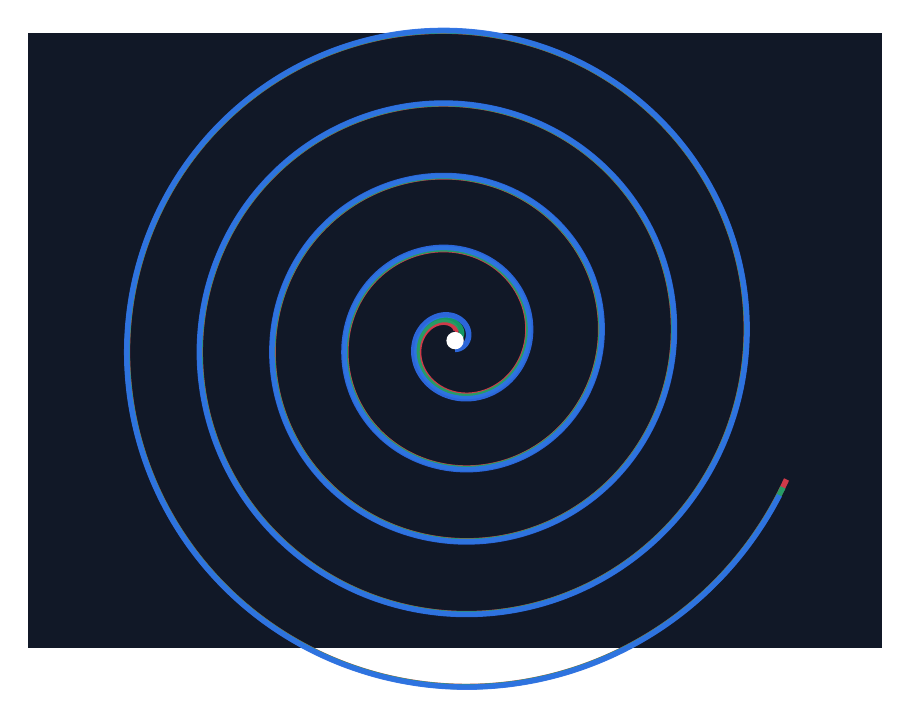
\begin{tikzpicture}[scale=.92]
\fill[Deep] (-5.9,-4.25) rectangle (5.9,4.25);
\draw[PR,line width=2.0pt,opacity=.9] plot[smooth,domain=0:31,samples=700] ({.16*\x*cos(\x r)-.12*sin(\x r)},{.16*\x*sin(\x r)+.12*cos(\x r)});
\draw[PG,line width=2.0pt,opacity=.9] plot[smooth,domain=0:31,samples=700] ({.16*\x*cos(\x r)},{.16*\x*sin(\x r)});
\draw[PB,line width=2.0pt,opacity=.9] plot[smooth,domain=0:31,samples=700] ({.16*\x*cos(\x r)+.12*sin(\x r)},{.16*\x*sin(\x r)-.12*cos(\x r)});
\fill[white] (0,0) circle (.12);
\end{tikzpicture}
\caption{Three normal-offset colour paths form one perceptually unified spiral.}
\end{figure}

\section{Density, strength and colour separation}
\subsection{Pattern-specific density semantics}
\begin{tabularx}{\linewidth}{@{}>{\bfseries}p{39mm}p{36mm}p{27mm}X@{}}
\toprule
Pattern & Displayed density & Default at 1600 px & Interpretation \\
\midrule
Vertical stripes & Number of stripes & 14 & Larger value produces more, narrower periods. \\
Horizontal stripes & Number of stripes & 14 & Same semantics after axis transposition. \\
Diagonal stripes & Number of stripes & 18 & Compensation accounts for diagonal geometry. \\
Halftone & Dot spacing & 12 px & Smaller spacing creates more dots. \\
Hexagonal halftone & Dot spacing & 12 px & Nearest-neighbour lattice pitch. \\
Spiral stripes & Turn spacing & 19 px & Radial distance between successive turns. \\
\bottomrule
\end{tabularx}

The adaptive preset system uses 1600 px as a reference and rescales pattern profiles when output size changes. This keeps the default geometry useful across low- and high-resolution exports rather than exposing internal renderer constants.

\subsection{Strength}
Strength $S$ is not a conventional brightness control. It multiplies local channel intensity before the clipping and width/area transfer function. Increasing it expands structures, raises average occupancy and improves visibility in dark regions, but may merge neighbouring elements. Decreasing it reveals more negative space and makes the near-field pattern more graphic.

\subsection{Colour separation}
Small separation values reconstruct neutral colours quickly at distance. Larger values create stronger cyan, magenta and yellow fringes and a more chromatic close-up appearance. Very large separation can reduce local correspondence between channels; the most useful value therefore depends on density.

A dimensionless way to compare separation across patterns is
\begin{equation}
\eta=\frac{d}{P_{\mathrm{local}}},
\end{equation}
where $P_{\mathrm{local}}$ is stripe period, dot spacing or spiral turn spacing. Equal pixel offsets do not have equal visual impact when density changes; the ratio $\eta$ explains why.

\section{Density animation}
\subsection{Parameter interpolation}
A density animation evaluates the renderer at a sequence of parameter values between $q_0$ and $q_1$. With normalised time $u=t/T$,
\begin{equation}
q(t)=q_0+E(u)(q_1-q_0),
\qquad 0\le t\le T,
\end{equation}
where $E$ is the selected easing function. For linear easing,
\begin{equation}
E(u)=u.
\end{equation}

Ping-pong playback maps time to a triangular phase:
\begin{equation}
E_{\mathrm{pp}}(u)=1-\left|1-2u\right|,
\qquad 0\le u\le 1,
\end{equation}
so the parameter travels to the end value and returns without a discontinuous reset.

\subsection{Reference animation profiles}
\begin{tabularx}{\linewidth}{@{}lcccX@{}}
\toprule
Pattern & Start & End & Default timing & Visual effect \\
\midrule
Vertical & 8 & 24 & 4.00 s at 12 FPS & Coarse to fine stripe field. \\
Horizontal & 8 & 24 & 4.00 s at 12 FPS & Coarse to fine horizontal field. \\
Diagonal & 10 & 28 & 4.00 s at 12 FPS & Increasing diagonal frequency. \\
Halftone & 24 px & 7 px & 4.00 s at 12 FPS & Large sparse dots to fine dense dots. \\
Hexagonal & 24 px & 7 px & 4.00 s at 12 FPS & Same progression on a hexagonal lattice. \\
Spiral & 24 px & 6 px & 4.00 s at 12 FPS & Wide to tightly spaced turns. \\
\bottomrule
\end{tabularx}

At frame rate $f$ and duration $T$, the nominal frame count is
\begin{equation}
N_f\approx fT.
\end{equation}
Higher FPS improves motion smoothness but increases generation time and file size. Preview at modest output size before exporting a high-resolution animation.

\section{Export, print and viewing geometry}
\subsection{Still-image export}
Percepta supports high-resolution still export for raster and document-oriented workflows, including PNG, TIFF, SVG and PDF in the current distribution. Raster formats preserve the exact rendered pixel geometry; vector/document exports are useful for placement in design or print workflows, subject to the capabilities of the selected pattern and backend.

\subsection{Pixel pitch and physical pitch}
For an output $N$ pixels wide printed at physical width $W$ millimetres, a geometric pitch of $p_{\mathrm{px}}$ pixels becomes
\begin{equation}
p_{\mathrm{mm}}=W\frac{p_{\mathrm{px}}}{N}.
\end{equation}
At viewing distance $d$ millimetres, the small-angle approximation gives
\begin{equation}
\alpha\approx\frac{p_{\mathrm{mm}}}{d}\quad\text{radians}.
\end{equation}
Expressed in arcminutes,
\begin{equation}
\alpha_{\mathrm{arcmin}}\approx3437.75\frac{p_{\mathrm{mm}}}{d}.
\end{equation}
These equations are more useful than a universal viewing-distance rule: the same digital file behaves differently when displayed on a phone, monitor, poster or fine-art print.

\subsection{Print checklist}
\begin{itemize}
\item Export at the final aspect ratio and sufficient pixel dimensions; avoid enlarging a low-resolution render after export.
\item Disable automatic sharpening when it creates halos around coloured edges.
\item Use a colour-managed workflow when colour fidelity matters.
\item Test a small crop at final physical size before producing a large print.
\item Evaluate under the intended illumination and at several distances.
\end{itemize}

\section{Practical recipes and troubleshooting}
\subsection{Starting recipes}
\begin{tabularx}{\linewidth}{@{}>{\bfseries}p{32mm}p{35mm}p{25mm}X@{}}
\toprule
Source & Suggested pattern & First adjustment & Reason \\
\midrule
Portrait & Vertical or halftone & Moderate separation & Preserves facial masses while retaining graphic texture. \\
Landscape & Horizontal or hexagonal & Lower contrast if sky clips & Horizontal structure follows natural layers. \\
Architecture & Diagonal or vertical & Increase output size & Straight edges benefit from finer sampling. \\
High-detail illustration & Hexagonal halftone & Reduce dot spacing & Isotropic lattice handles detail in several directions. \\
Abstract image & Spiral & Move centre deliberately & Centre placement becomes part of the composition. \\
\bottomrule
\end{tabularx}

\subsection{Common problems}
\begin{tabularx}{\linewidth}{@{}>{\bfseries}p{38mm}X@{}}
\toprule
Symptom & Corrective actions \\
\midrule
The source is not recognisable at any scale & Increase strength; reduce source contrast if highlights or shadows are clipped; use finer density; try halftone for high-detail material. \\
The result looks almost solid & Reduce strength, increase dot or turn spacing, or reduce stripe count. \\
Colours look excessively split & Reduce colour separation, especially at fine density. \\
Dark regions vanish & Increase strength or the halftone minimum size; reduce source contrast. \\
Lines or spiral look noisy & Increase line/path smoothing or use a lower-contrast source. \\
Animation flickers & Increase FPS, reduce the parameter range, or choose gentler easing. \\
Export is slow & Test at a smaller output size, then generate the final file once settings are stable. \\
\bottomrule
\end{tabularx}

\section{Implementation notes and limits}
\subsection{Sampling and complexity}
For an $N\times N$ output, image preparation is $\mathcal{O}(N^2)$. Stripe rendering combines $\mathcal{O}(N^2)$ rasterisation with a number of local profiles proportional to stripe count. Halftone cost grows with the number of cells, approximately $(N/p)^2$. Spiral cost is dominated by path samples and line rasterisation; path sample count is selected from the estimated arclength and bounded for predictable memory use.

\subsection{What the model does not guarantee}
\begin{itemize}
\item Exact colourimetric reconstruction after printing; inks, paper and colour management alter additive RGB assumptions.
\item A fixed fusion distance for all observers and devices.
\item Preservation of every high-frequency source feature; encoding is intentionally spatially lossy.
\item Equivalent appearance across patterns at numerically equal density values; the units differ by design.
\end{itemize}

\subsection{Formula summary}
\begin{align}
L &=0.2126R+0.7152G+0.0722B,\\[3pt]
P_{\mathrm{stripe}}&=\frac{N}{n},\\[3pt]
w_c&=w_{\min}+(w_{\max}-w_{\min})\clip(S\widetilde I_c^{0.82},0,1),\\[3pt]
r_c&=\max\!\left(r_{\min},0.47p\sqrt{\clip(S\bar I_c,0,1)}\right),\\[3pt]
r(\theta)&=a+\frac{p}{2\pi}\theta,\\[3pt]
q(t)&=q_0+E(t/T)(q_1-q_0),\\[3pt]
p_{\mathrm{mm}}&=W\frac{p_{\mathrm{px}}}{N},\\[3pt]
\alpha_{\mathrm{arcmin}}&\approx3437.75\frac{p_{\mathrm{mm}}}{d}.
\end{align}

\section*{Credits and contact}
\addcontentsline{toc}{section}{Credits and contact}
Percepta was designed and developed by \textbf{Virgile Adam}. The software combines image processing, geometric rendering and perceptual presentation in a compact desktop workflow.

\begin{tabularx}{\linewidth}{@{}lX@{}}
\toprule
Author & Virgile Adam \\
Affiliation & IBS --- CNRS --- Universit\'e Grenoble Alpes \\
Email & \href{mailto:virgile.adam@ibs.fr}{virgile.adam@ibs.fr} \\
Website & \href{https://www.virgile-adam.com}{https://www.virgile-adam.com} \\
Project & \href{https://github.com/VirgileAdam/Percepta}{https://github.com/VirgileAdam/Percepta} \\
\bottomrule
\end{tabularx}

\vfill
\begin{center}
\RGBbar\\[5mm]
{\large\bfseries\color{Ink}PERCEPTA}\\[1mm]
{\small\color{Muted}Geometry carries colour. Distance reveals the image.}
\end{center}

\end{document}
